\documentclass{emulateapj}
%\documentclass{aastex}
\submitted{{\it Submitted for publication in ApJL}}
\usepackage{multirow,color,wrapfig,ulem}
\usepackage {graphicx}

\usepackage{amsmath} 
\usepackage{amssymb} 
\usepackage{graphics}
\usepackage{epsfig}  
\usepackage{float}
\bibliographystyle{apj}
\def\be{\begin{equation}}
\def\ee{\end{equation}}
\def\ba{\begin{eqnarray}}
\def\ea{\end{eqnarray}}

\newcommand{\avg}[1]{\langle{#1}\rangle}  
\newcommand{\hMpc}{{\ifmmode{h^{-1}{\rm Mpc}}\else{$h^{-1}$Mpc }\fi}}  
\newcommand{\hGpc}{{\ifmmode{h^{-1}{\rm Gpc}}\else{$h^{-1}$Gpc }\fi}}  
\newcommand{\hmpc}{{\ifmmode{h^{-1}{\rm Mpc}}\else{$h^{-1}$Mpc }\fi}}  
\newcommand{\hkpc}{{\ifmmode{h^{-1}{\rm kpc}}\else{$h^{-1}$kpc }\fi}}  
\newcommand{\hMsun}{{\ifmmode{h^{-1}{\rm {M_{\odot}}}}\else{$h^{-1}{\rm{M_{\odot}}}$}\fi}}  
\newcommand{\hmsun}{{\ifmmode{h^{-1}{\rm {M_{\odot}}}}\else{$h^{-1}{\rm{M_{\odot}}}$}\fi}}  
\newcommand{\Msun}{{\ifmmode{{\rm {M_{\odot}}}}\else{${\rm{M_{\odot}}}$}\fi}}  
\newcommand{\msun}{{\ifmmode{{\rm {M_{\odot}}}}\else{${\rm{M_{\odot}}}$}\fi}}  
\newcommand{\kms}{{\ifmmode{{\mathrm{\,km\ s}^{-1}}}\else{\,km~s$^{-1}$}\fi}}
\newcommand{\bullb}{MACS J0025.4-1222}
\newcommand{\bulla}{1E0657---56} 
\newcommand{\bullg}{SL2S J08544-0121}
\shorttitle{Bullet Groups}
\shortauthors{Fern\'andez-Trincado et al.}

\begin{document} 

\title{The abundance of Bullet-Groups in $\Lambda$CDM}
\author{J. G. Fern\'andez-Trincado$^{1,2,3}$, J. E. Forero-Romero$^1$,
  T. Verdugo$^3$, G. Foex$^4$ and V. Motta$^4$} 
\affil{$^1$ Departamento de F\'{i}sica, Universidad de los Andes,
  Cra. 1 No. 18A-10, Edificio Ip, Bogot\'a, Colombia\\ 
       $^2$ Institute Utinam, CNRS UMR6213, Universit\'e de
  Franche-Comt\'e, OSU THETA de Franche-Comt\'e-Bourgogne,
  Besan\c{c}on, France\\ 
       $^3$ Centro de Investigaciones de Astronom\'ia, AP 264,
  M\'erida 5101-A, Venezuela\\
  $^4$ Departamento de F\'isica y Astronom\'ia, Universidad de
  Valpara\'iso, Avda. Gran Breta\~na 1111, Playa Ancha, Valpara\'iso
  2360102, Chile  
}        

\begin{abstract}

We estimate the expected distribution of displacements between the two
dominant dark matter density peaks and between baryons and dark matter
in halos simulated within a full cosmological context. We use as a benchmark the
observation of \bullg, which is the lowest mass system observed so far
featuring a bi-modal dark matter distribution with a dislocated 
baryonic component. We extend previous results by
studying two halo samples: groups and clusters. We find that 50\% to 60\%
of the dark matter halos with circular velocities in the range
$300\kms$ to $700\kms$ (groups) show multimodal morphologies with
displacements between the dark matter clumps equal or larger than
$133\pm21$\hkpc as observed in \bullg. For dark matter halos with
circular velocities larger than $700\kms$ (clusters) this fraction
rises to $80\%$ to $85\%$. Using the same simulation we estimate the
dark matter-to-baryon spatial separation and find that $0.1\%$ to
$1.0\%$ of the groups should present separations equal or
larger than $87\pm 14$\hkpc corresponding to our observational
benchmark; for clusters this fraction is in the range of $4\%$ to
$10\%$, consistent with previous studies of dark matter to baryon
separations. The extension of the theoretical predictions and
observational results towards low mass Bullet-like configurations,
i.e. larger abundance of systems,  opens up the possibility for a new
statistical test of  $\Lambda$CDM.  
\end{abstract}

\begin{keywords}
{cosmology: theory -- dark matter} 
\end{keywords}

\section{Introduction}


The Bullet Cluster (\bulla) provided a new
kind of observational evidence for the existence of dark matter
\citep{Markevitch2004,Clowe2006}. Quantifying the displacement between
dark matter and the dominant baryonic component (hot X-ray emitting gas)
has been used to test the Cold Dark Matter (CDM)
paradigm itself by quantifying the substructure velocity required to
produce such displacement \citep{Hayashi2006, Springel2007,
  Thompson2012}, the displacemeent between the dominant dark matter
and baryonic component \citep{ForeroRomero2010} to estimate the
expected abundance of such events in a $\Lambda$CDM Universe and even
explore possible extensions to the concordance cosmological model
\citep{Farrar2007,Lee2010,Lee2012}.    


Since then, other examples of Bullet-like systems have been found; 
MACS J0025.4-1222 \citep{Bradac2008}, Abell 2744 \citep{Merten2011},
DLSCL J0916.2+2951 \citep{Dawson2012}, ZwCl 1234.0+02916
\citep{Dahle2013}. Recently \citep{Gastaldello} observed a baryonic-DM
displacement if $124\pm 20$ kpc in \bullg, a group-like system with a total
mass $2.4\pm 0.6 \times 10^{14}$\Msun. Systems of this mass are
$\sim10$ times more abundant than cluster systems in the mass range of
the Bullet Cluster $>10^{15}$\hMsun, this opens up the possibility of
observationally finding bullet groups in a fair amount to impose
constraints on $\Lambda$CDM. 


However, a greater abundance of small mass systems has to be weighted
by the probability of having a merger and 
presenting a large displacement between the DM and baryonic
components. These two conditions (merger rates, maximum possible
displacement) are a funcion of halo mass in $\Lambda$CDM
cosmologies.  Such study has been performed for clusters but not for
lower mass systems \citep{ForeroRomero2010}. The existence of objects
like \bullg and observational campaigns like the Strong Lensing Legacy
Survey (SL2S) open up the possibility of finding multi-modal dark
matter distributions in the group mass range.


In this Letter we compute the abundance of group-like dark
matter halos with a multi-modal morphology that also might present a
DM-baryon displacement. To this end we use a N-body cosmological
simulation with such a resolution that allows us to identify
multi-modal dark matter distributions in hosts with circular velocities
larger than $300$\kms.  

This Letter is organized as the follows. In Section
\ref{sec:simulation} we present the simulation and the halo catalogs
used in this work. We continue in Section \ref{sec:setup} with the
geometry of the problem at hand and the measurements setup. Next in
Section \ref{sec:results} we present our results and observational
perspectives to finally conclude in Sections \ref{sec:conclusions}. 


\section{Simulation, halo catalogs and pairs}
\label{sec:simulation}

We use the Bolshoi Run, a cosmological DM only simulation over a cubic
volume of 250\hMpc comoving on a side. The simulation uses the ART code to
follow the evolution of a dark matter density field sampled with
$2048^3$ from $z=80$ to $z=0$. The cosmology used  corresponds
to  the spatially flat concordance model with the following
parameters:  the density parameter for matter (dark matter and baryons)
$\Omega_m=0.27$, the density parameter for baryonic matter
$\Omega_b=0.0469$, the density parameter for dark energy
$\Omega_{\Lambda}=0.73$, the Hubble parameter $h=0.7$, the
normalization of the Power spectrum $n=0.95$ and the amplitude of mass
density fluctuation (at redshift z$=$0) $\sigma_8=0.82$.  These
cosmological parameters are consistent with the nine-year Wilikinson
Microwave Anisotropy Probe (WMAP) results \citep{hinshaw_etal13}. A
detailed presentation of the simulation can be found in
\citet{2011ApJ...740..102K}.     


The number of particles used for each of the DM component was
$2048^3$, resulting in a mass resolution of $1.35 \times 10^8$
M$_{\odot}$h$^{-1}$. The completeness limit in this simulation is set
for halos with $100$ particles corresponding to a mass of
$1.35\times10^{10}$\hMsun or a maximum circular velocity $V_{c}$ of
$50$\kms. 

We use halo catalogs constructed using the Bound Density Maxima (BDM)
algorithm \citep{BDM,BDMb}. To define the radius of a halo we use a
density threshold of 360 times the mean density of the Universe, for 
different redshifts we use the overdensity criterion by
\cite{Bryan1998}. An important feature of BDM is that it allows us to
detect sub-halos inside larger virialized structures. 


All the raw data used in this Letter is
available through the Multidark database \footnote{\texttt{www.multidark.org}}
\citep{Riebe2013}.  Furthermore, in order to facilitate the
reproducibility and reuse of our results we have made available all
the data and the source code available in a public
repository \footnote{\texttt{https://github.com/Fernandez-Trincado/Bullet\_Groups-2014}}.

In this Letter we make a study at four different redhifts $z=0.0,0.25,
0.5$ and $1.0$. First, we select all the host halos (i.e. halos that
are not inside a larger halo) with circular velocities $V_{\rm c}\geq
300$\kms. Then, we select the sub-halos with circular velocities
$V_{\rm c}\geq 75$\kms. The objective is to use this sub-halos as the
tracer of the sub-dominant dark matter clump in the merging cluster,
i.e. the bullets.

For the redshifts $z=0.0,0.25, 0.5$ and $1.0$ we find $10041, 10346,
10554$ and $10382$ host halos and $157853, 177331, 195072, 225188$
sub-halos, respectively. These two sets (host halos and sub-halos)
constitute the basis for our analysis. We find now for each host halo
we its most massive sub-halo. Each pair host halo/sub-halo is
considered as a potential Bullet system and is kept for the analysis
described in the next Section.  

\section{Bullet Geometry and Measurement Setup}
\label{sec:setup}

The Bullet-like configurations are composed by two dark matter
structures: the host halo and the dominant sub-halo. We describe the
kinematics of this configuration by the 
position and velocity vectors of the sub-halo in a frame of reference
where the main halo is at rest; thus
$\vec{v{}}=\vec{v}_{sub}-\vec{v}_{halo}$ and
$\vec{r}=\vec{r}_{sub}-\vec{r}_{halo}$, where the subscripts $host$
and $sub$ refer to the position of the minium of potential for the
host and sub-halo in the frame of reference of the simulation,
respectively.  

The angle between these two vectors can be characterized by, 
\begin{equation}
  \mu\equiv
  \cos(\theta)=\frac{\vec{v{}}\cdotp{}\vec{r}}{\left\|\vec{v}{}\right\|
    \left\|\vec{r}\right\|} .
 \end{equation} 
%
This encodes relevant information to describe the collision,
i.e. cases of $|\mu|\approx 1$ can be considered as head-on collisions
while $|\mu|\approx 0$ describes a grazing trajectory.

The geometrical configuration can be further described by the
following quantities. The circular velocity of each component, $V_{\rm
  c,host}$ for the host and $V_{\rm c, sub}$ for the sub-halo and the
size of the host halo $R_{\rm vir}$. Another useful quantity computed
in the simulation is the distance between the minium of potential for
the host halo and its center of mass, $X_{\rm
  off}=||\vec{r}_{min}-\vec{r}_{cm}||/R_{\rm vir}$ which serves as a
measurement of how perturbed is the host halo.

As a zero-th order approximation, in this paper we work with three
quantities that are available from observations of Bullet-like
systems. The projected distance between two dominant DM clumps, the
projected distance between the DM-baryonic clumps and the ratio of the
mass associated to the DM clumps.  

From the simulation point of view, the first quantity can be
translated into the 2D projected values of $||\vec{r}||$ and its value
relative to the virial radius $D_{\rm   off}= ||\vec{r}||_{\rm
  2D}/R_{\rm vir}$. The last quantity, the mass ratio, can be
approximated by ratio of the circular velocities of the two clumps $V_{\rm c,sub}/V_{\rm  c,host}$ which should be equal to the square root of the mass
ratio. The second quantity, the projected DM-baryon distance, is not
directly available from a DM-only simulation but, as we show in the
Results section, can be inferred from the available information.  
 


In order to gain better insight, we use two
quantities that are not readily available from observations but can be
measured in the simulation. The first one is the sub-structure
velocity as a fraction of the host's circular velocity, $||\vec{v}||/V_{\rm c, host}$, as a measure of the the strength of the
merger.  The second is $\mu$ to measure the geometry (head-on
vs. grazing) of each collision.


The physical quantities described above can be used to describe
the three main stages in a bullet-like encounter. First, the sub-halo
crosses the virial radius of the host halo starting a head on
collision, $||\vec{r}||/R_{\rm vir}\approx 1$ and
$\mu\approx<0.0$. Second, as the sub-halo crosses for the first time
the center of the host halo $||\vec{r}||/R_{\rm vir} < 1.0$ and
$\mu>0.0$. Third, as the sub-halo reaches apogee and comes back to the
center of the halo $||\vec{r}||/R_{\rm vir} < 1.0$ and $\mu<0.0$. We use
this quantities in the enxt section to fully characterize the different
kind of interactions observed in the Bolshoi Run,


\section{Results}
\label{sec:results}

\subsection{Displacements and Relative Circular Velocities}
\label{fig:displacement}

\begin{figure*}
\begin{center}
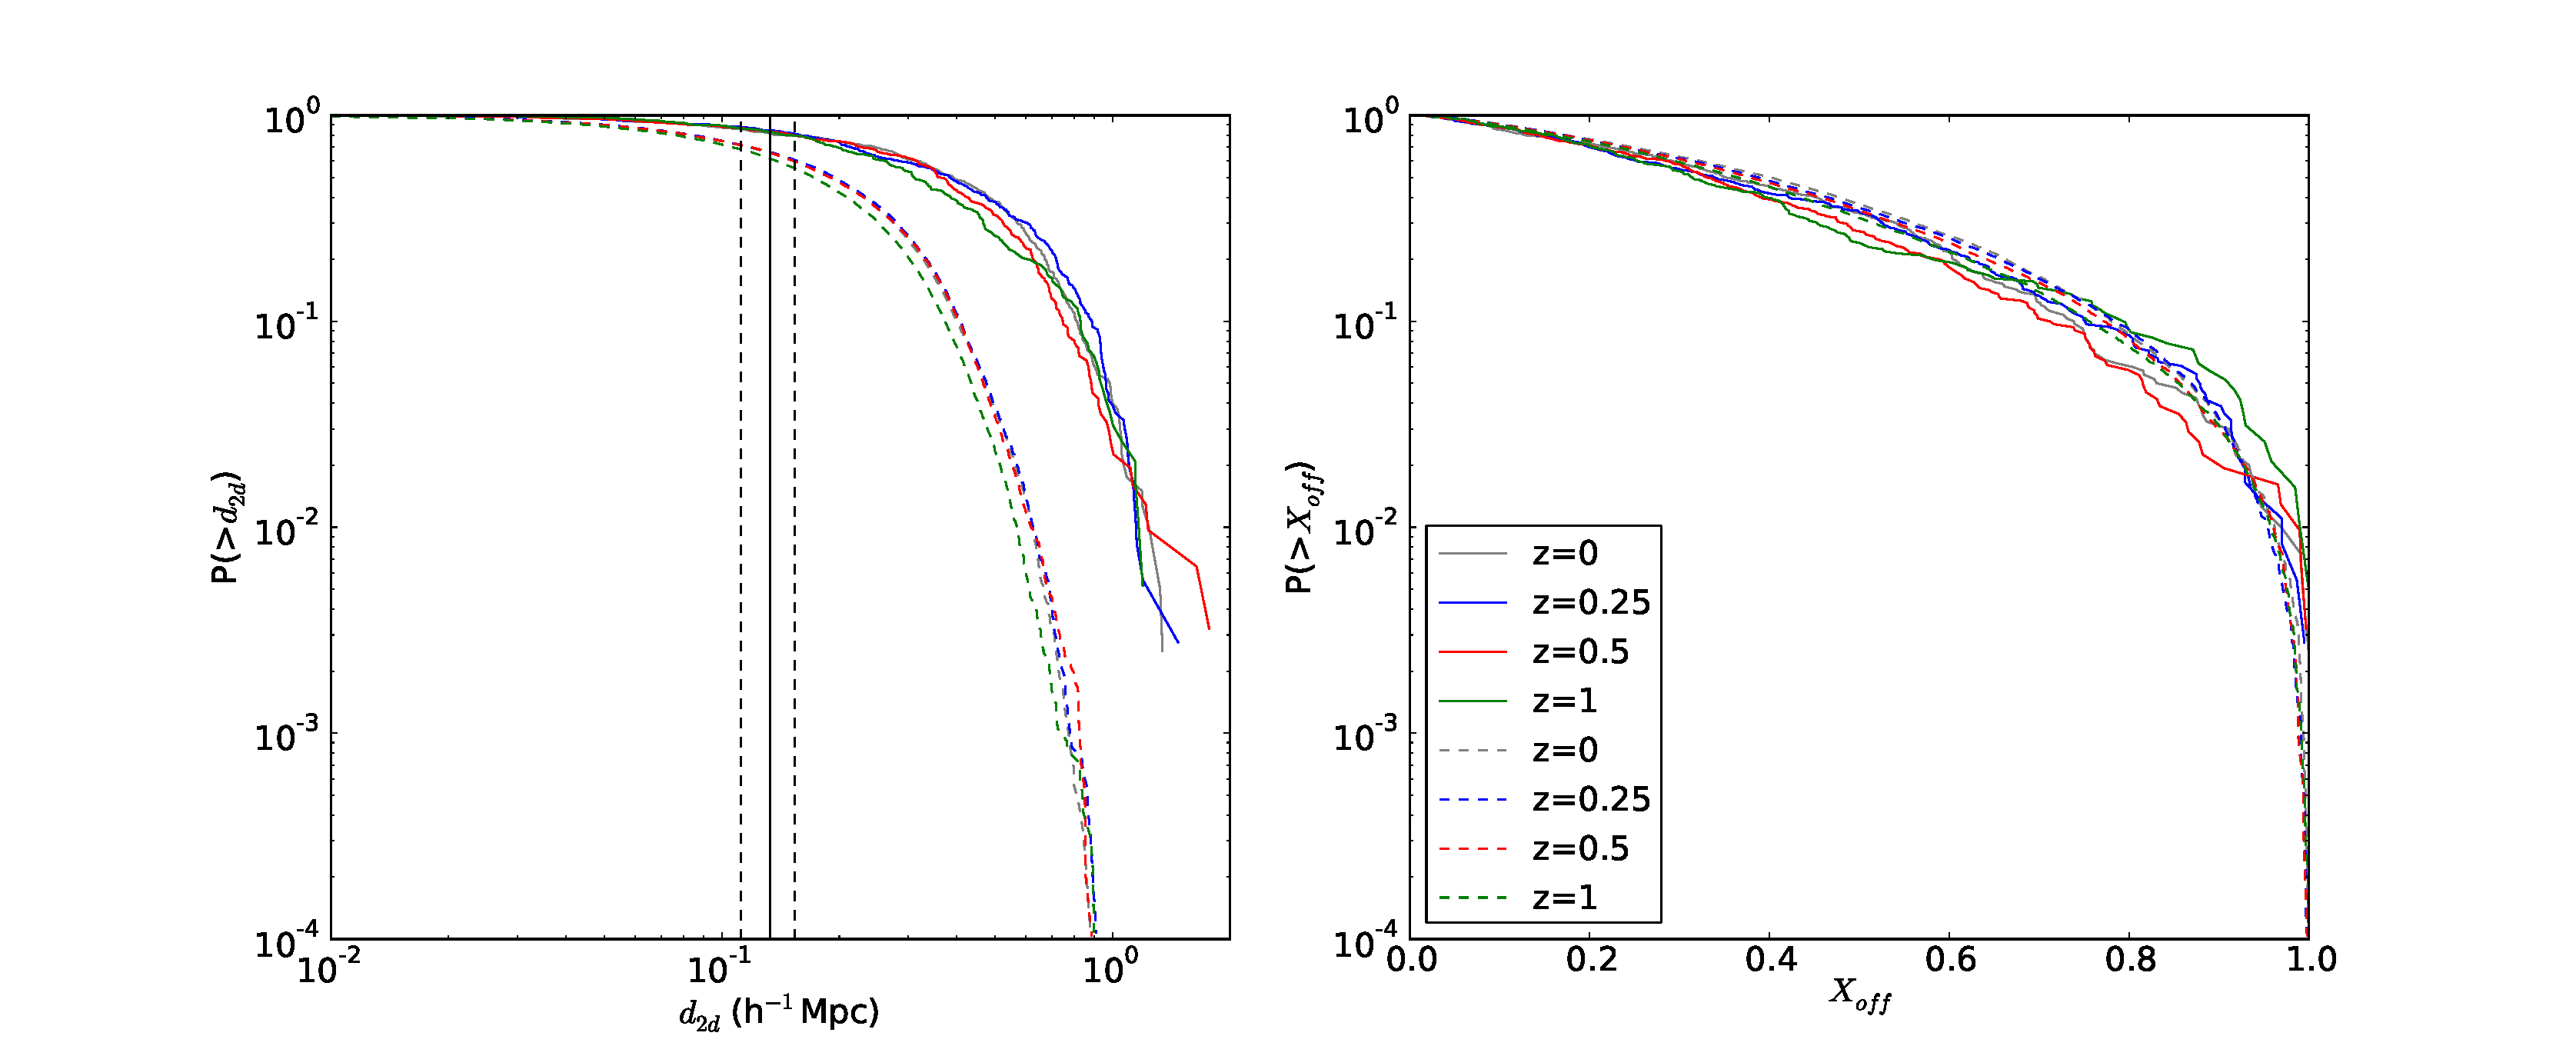
\includegraphics[width=0.9\textwidth]{figure_1.eps}
\end{center}
\caption{
  Integrated probability distribution for the displacement
  between the center of the host halo and its dominant sub-halo. The left panel
  shows the results in terms of the physical displacements while
  the right panel shows the displacements normalized by the virial radius of
  the host halo. The continuous (dashed) line corresponds to the halos in the
  cluster (group).
  The vertical lines shows the mean and uncertainties in the estimated
  separation  between the two dark matter clumps in the results reported by
  \citet{Gastaldello} for the \bullg. Between $50\%$
  to $60\%$ of the groups show a displacement equal or larger than
  this observational benchmark.}
\label{fig:displacement}
\end{figure*}

\begin{figure*}
\begin{center}
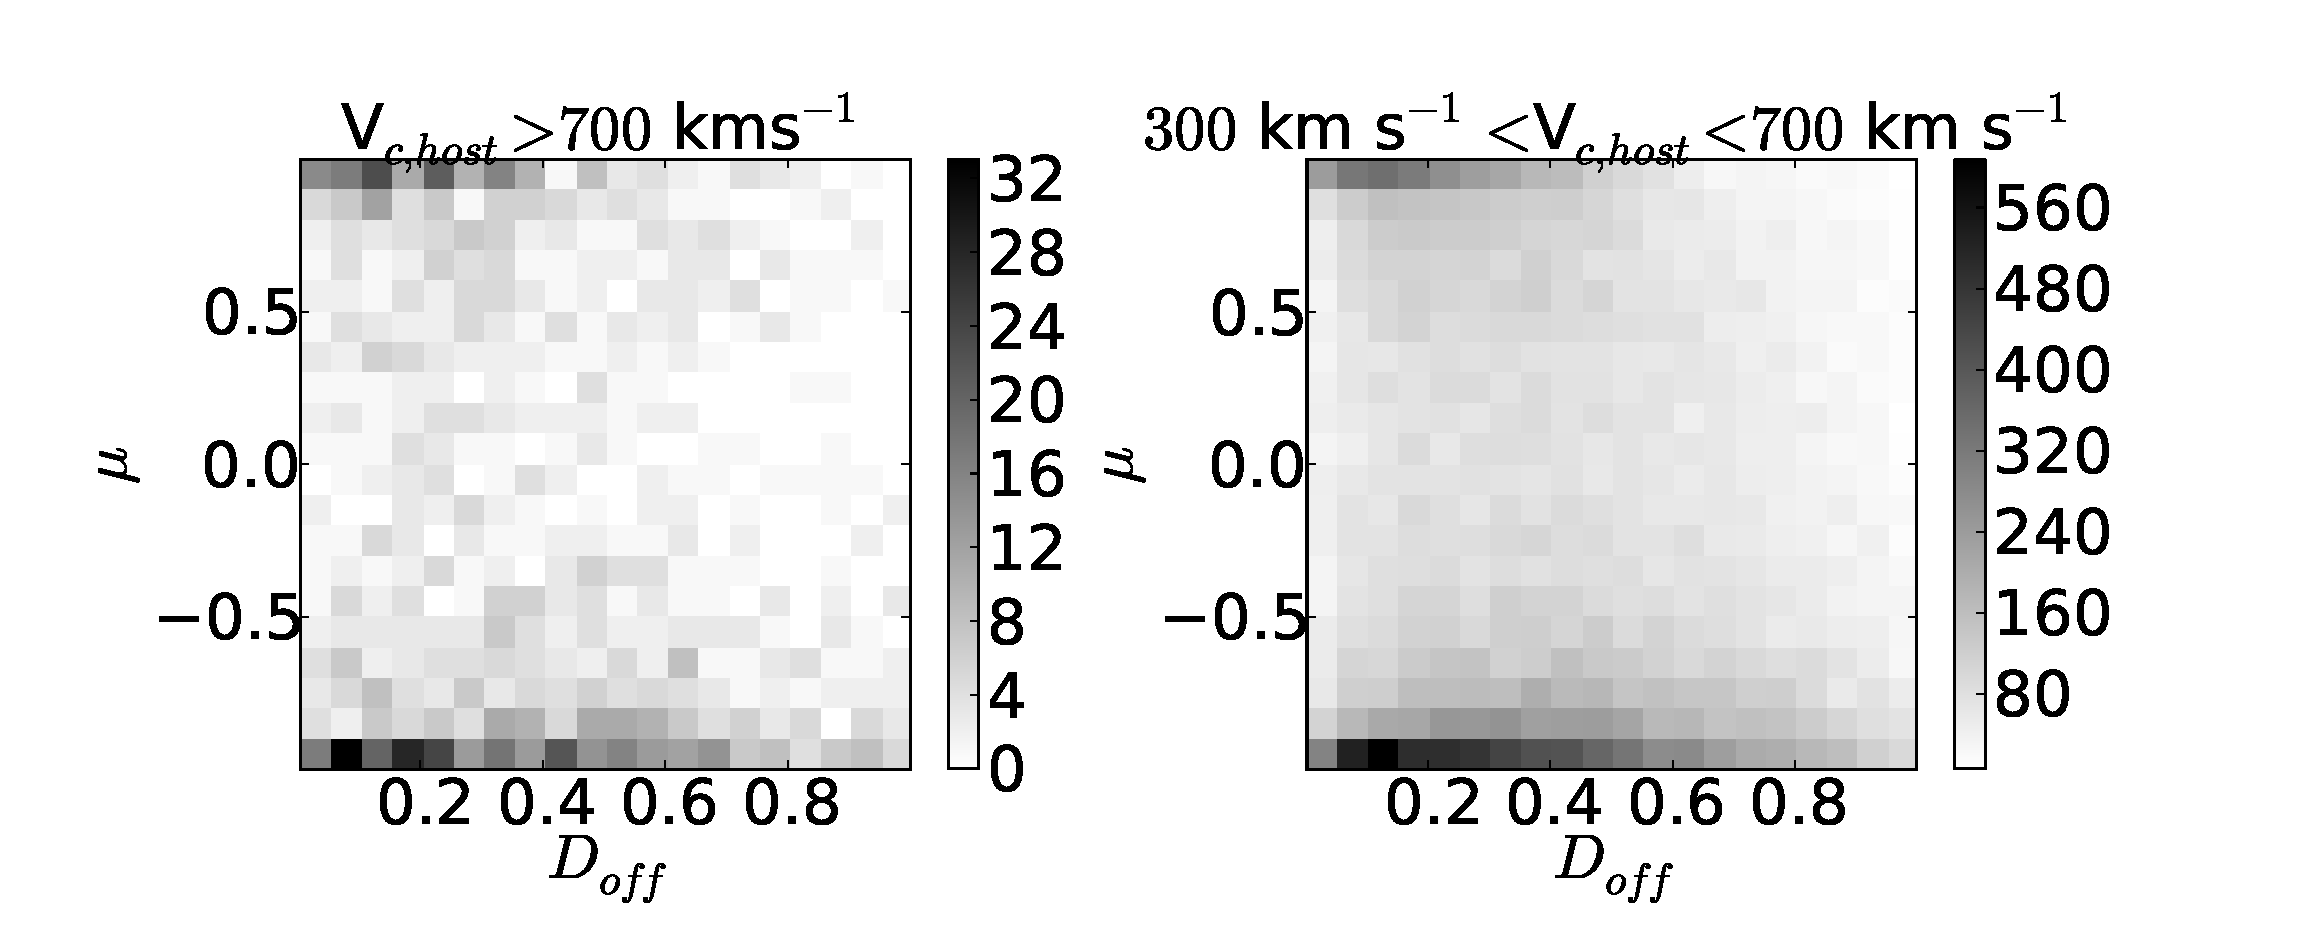
\includegraphics[width=1.0\textwidth]{figure_2.eps} 
\end{center}
\caption{2D histogram in the plane $V_{\rm c,sub}/V_{\rm
    c,host}$-$d_{2D}$. The left panel corresponds to clusters and the
  right panel to groups. The star with error bars corresponds to
  \bullg data reported from \citet{2013A&A...552A..80M} and
  \citet{Gastaldello}. The data used to construct the histograms
  integrates the objects at all redshifts. }
\label{fig:mass_displacement}
\end{figure*}

The main result of this paper is summarized in Figure
\ref{fig:displacement}, it presents the integrated
probability distribution for the displacement between the center of
the host halo and its dominant sub-halo. The left panel shows
the displacement in physical units and the right panel as a fraction
of the virial radius of the host halo. 

Figure \ref{fig:displacement} shows the results for two different
populations; groups with $300\kms < V_{\rm c, host}<700\kms$ and
clusters with $V_{\rm c,host}>700\kms$. Additionally, this is
presented for all redshifts $z=0.0, 0.25, 0.5$ and $1.0$. 

The panel with the projected 2D physical displacements also shows a
vertical stripe with the estimated displacement for the Bullet-group reported by
\cite{Gastaldello}. In the group sample we see that a fraction of
$50\%$ to $60\%$  should present a displacement equal than the
estimate for \bullg; in the cluster sample this fraction increases to
$80\%$-$85\%$. This fraction is naturally higher in more massive
systems because they are larger in size. Normalizing the displacements
by the virial radius, right panel Figure \ref{fig:displacement}, we
see that the distribution is the same regardless of the sample and the
redshift.

Figure \ref{fig:mass_displacement} shows 2D histograms in a plane
defined by the ratio of the two circular velocities $V_{\rm c,
  sub}/V_{\rm c, host}$ and the projected 2D physical displacements;
quantities that can be constrained by observations. The displacement
is a direct observable, while the ratio of the circular velocities can
be estimated from lensing studies or approximated by the ratio of the
total galaxy luminosity associated with the galaxy peaks or by a
lensing reconstruction. 

To construct this figure we co-add all the halos in the sample (left,
clusters; right, groups) at all redshifts. We stack the data because
we do not observe any strong redshift dependence, additionally this allows
us to increase the signal in each bin. We overplot a star with error
bars that represents the observational estimates for the system
\bullg\ using the fraction in velocity dispersion in the line-of-sigth
of the group SL2S SJ08544-0121 ($\sigma_{host}=341^{+43}_{-109}$\kms and
$\sigma_{sub}=185^{+30}_{-62}$\kms) reported by
\citet{2013A&A...552A..80M} and the DM displacement inferred from the
data presented by \cite{Gastaldello}.  


\subsection{Relative Velocities}
\label{sec:velocities}

\begin{figure*}
\begin{center}
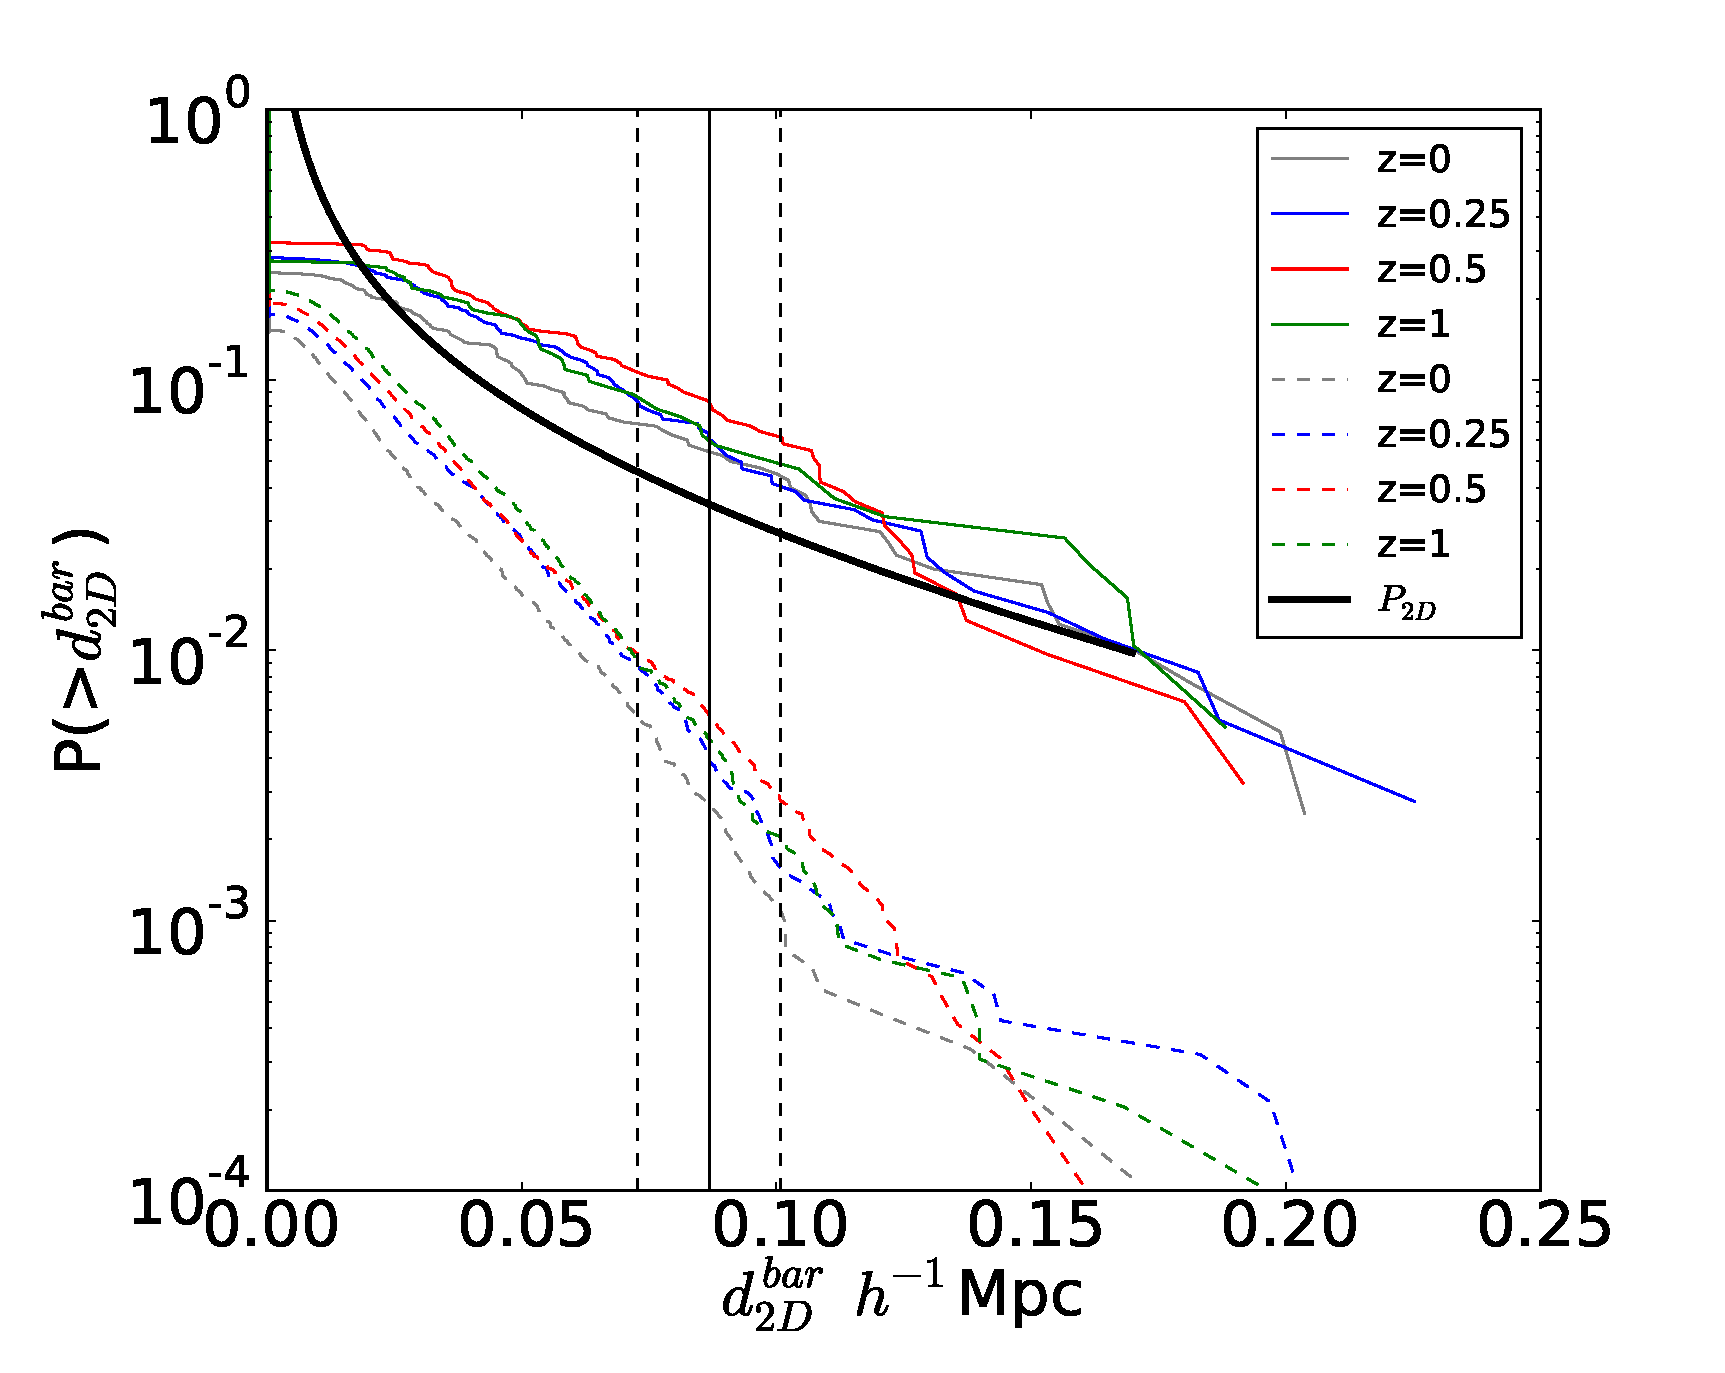
\includegraphics[width=0.9\textwidth]{figure_3.eps}
\end{center}
\caption{Integrated probability distribution for the relative velocity of the
sub-halo with respect to its host. The left panel shows the results
in physical units while the right panel show the same values
normalized by the circular velocity of the host halo. The line encoding
follows the same structure as Figure \ref{fig:displacement}}
\label{fig:velocities}
\end{figure*}


\begin{figure*}
\begin{center}
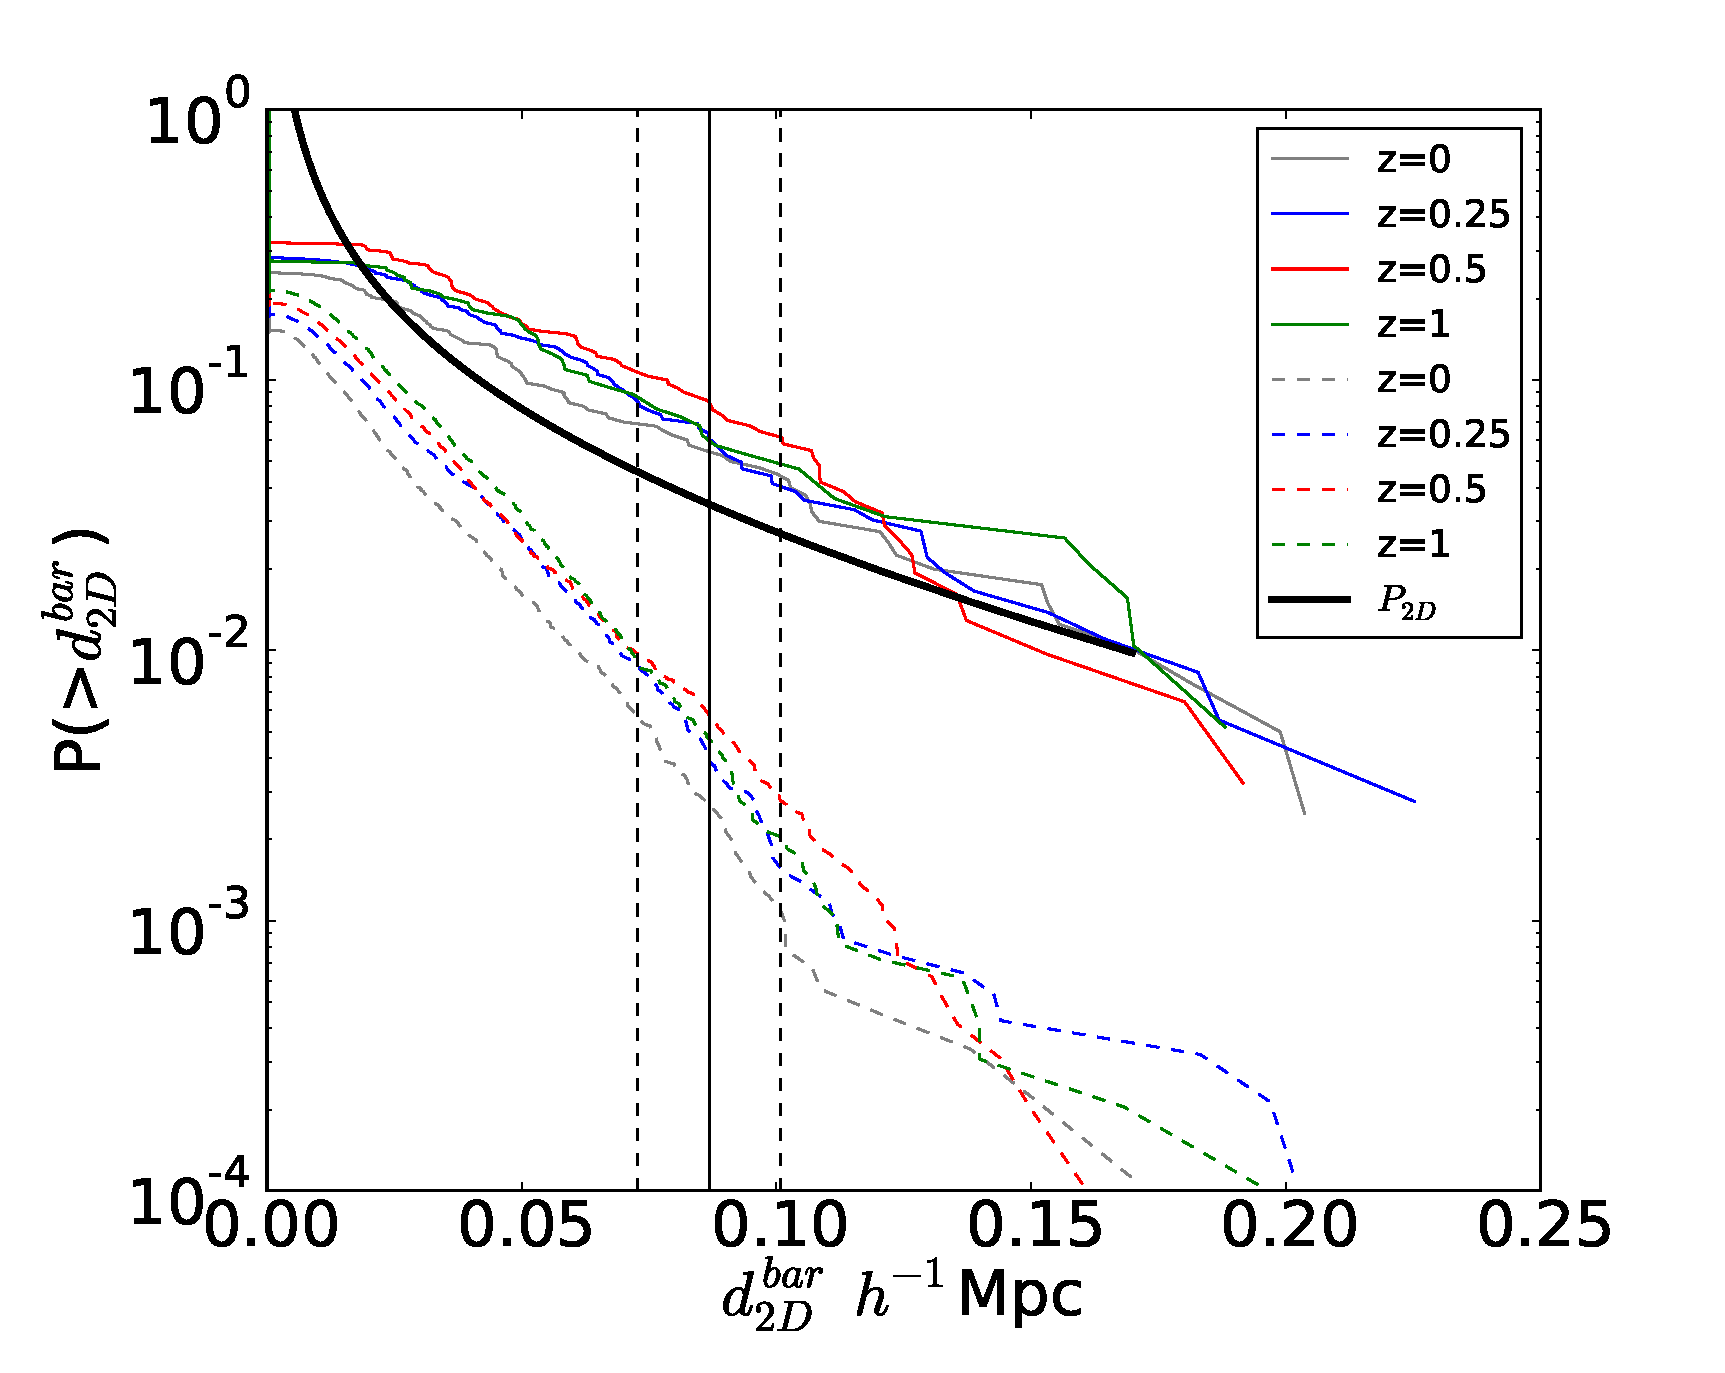
\includegraphics[width=1.0\textwidth]{figure_4.eps}
\end{center}
\caption{2D histograms in the plane $\mu$-$D_{\rm off}$. The left
  panel corresponds to clusters and the right panel to groups. The data
  used to construct this histogram includes the halos at all redshifts.}
\label{fig:geometry}
\end{figure*}


In Figure \ref{fig:velocities} we present the integrated probability
of the relative peculiar velocities of the sub-halos with respect to
the host halo. The left panel presents this velocity in physical units
while the right panel presents them as a fraction of the circular
velocity of the host halo.  

The panel with the normalized velocities shows that the distribution
of sub-halo velocities is close to universal. Regardless of the mass
of the host halo and the redshift the integrated distributions lie
very close to each other.  The universality of this profile extends to
the group mass range the findings of \citep{Hayashi2006} for clusters.

The median of this distribution is located at $v/V_{\rm
  c,host}=1.1$. We also note the strong break at $v/V_{\rm
  c,host}=3.0$ that is present in the data from the group sample that
allows us to probe fractions on the order of $10^{-4}$.  This break is
located close the escape velocity of $v/V_{\rm c,host}$ for dark
matter halos following a NFW profile with a concentration value
$c\approx 6$ \citep{Hayashi2006}.  





\subsection{Collision Geometries}
\label{fig:geometry}

Figure \ref{fig:geometry} presents the geometry of the bullet groups using the 
variables $\mu$ and $D_{\rm off}$. The first evident feature is that
most of the configurations have $|mu|>0.9$ ($\theta\leq 30^{\circ}$),
meaning that most of the collisions can be described as a head-on
encounter while only a minority with $|mu|<0.9$ have grazing
trajectories. For the pairs on radial trajectories there are three
regions of interest in this plane that describe different stages in
the collision, assuming that the sub-halo merges (or falls below the
BDM detection threshold) right at its second pass through the center
of the host halo \citep{Poole2006}.  


The first region has $\mu\approx-1$ and $D_{\rm off}>0.6$, which
locates the systems where a head-on collision has just started. The
sub-halo is close to the boundary of the host halo and is
infalling. The second region has $\mu\approx 1$ and $D_{\rm off}<0.6$;
at this stage the collision continues after the first crossing of the
host's center, the low number of halos with radial infalling velocities
and displacements $D_{\rm off}>0.6$ suggest that this the maximum
range of radii for the apogee.  The third region corresponds to
$\mu\approx-1$ and $D_{\rm off}<0.6$ which corresponds to the
secondary infall after apogee. We use this sequence in the next
subsection to estimate the expected displacement between baryons and
the dominant DM clump. 



\subsection{Displacement between Dark Matter and Baryons}
\label{sec:baryonic_displacements}



Strictly speaking, the results we have derived so far, apply to multi-modal
groups and their expected separation between the two dominant dark
matter clumps. These displacements cannot be interpreted that all have a
corresponding DM-baryon displacement. 


However, these different stages for a collision, that we describe at
the end of the previous sub-section, can produce different results in
terms of the displacement between dark matter and baryons. For
instance, the systems where the halo is starting to fall into the host
($\mu\approx-1$, $D_{\rm off}>0.6$) should not present a detectable
DM-baryon displacement.  We do expect such displacements when the
sub-structure has already passed through the center of the host halo,
i.e. cases where $\mu\approx 1$. 

In this sub- section we estimate DM-baryon displacement statistics. We
work under the following hypothesis. First, we consider that systems
with $|\mu|<0.9$ have a baryonic displacement, $d_{2D}^{\rm bar}$,
equal to zero. This means that only head-on encounter produce a
displacement. Second, we consider that all systems with infalling
velocities $\mu<-0.9$ and large displacements $D_{\rm off}>0.6$ also
have baryonic displacements equal to zero. Third, for all the other
cases we estimate the displacement between the baryons and the
dominant DM peak by the distances between the dominant peak and the
center of mass of the main halo, $d_{2D}^{\rm bar} = X_{\rm off} R_{\rm
  vir}$, where $X_{\rm off}$ is the offset computed between the minium
of potential and the center of mass for each host halo.


This simplified model does not take into account that there is a
fraction of halos with $\mu<-0.9$ and $D_{\rm off}<0.6$ for which the
collision has not started and should have $d_{2D}^{\rm bar}=0$. A detailed
modeling of this fraction requires the study of the complete merger
tree of the halo and sub-halo, a study beyond the scope of this
Letter. Instead we caution the reader that the derived fraction of
halos with a displacement $<d_{2D}^{\rm bar}$ can be considered as an
upper limit. 

The results for the integrated distributions for $>d_{2D}^{\rm bar}$
are shown in Figure \ref{fig:baryonic_displacements}. The dashed lines
represented the results for groups and the continuous lines correspond
to clusters. As a test of our approach we compare the cluster results
against the analytic fit provided by \cite{ForeroRomero2010}. This fit
reproduces the statistics for the DM-baryon separation found for
clusters more massive than $>10^{14}$\hMsun in a simulation
that included a description for gas with $8$ times the volume of the
Bolshoi Simulation. The fit is valid for separations larger than
$70$\hkpc, beyond which we find that it provides a remarkably good
description within a factor of $\sim 2$ of our results. This gives us
confidence in our approach to estimate the expected fraction of
groups with a DM-baryon displacement.

From Figure \ref{fig:baryonic_displacements} we see that only a
fraction of $0.1\%$ to $1\%$ of the groups are expected to have a
DM-baryon displacement equal or larger than $87\pm 14$\hkpc as
observed in \bullg. This fraction rises to $4\%$ to $10\%$ in the case
of clusters, consistent with the results reported by
\cite{ForeroRomero2010}. 



\begin{figure}
\begin{center}
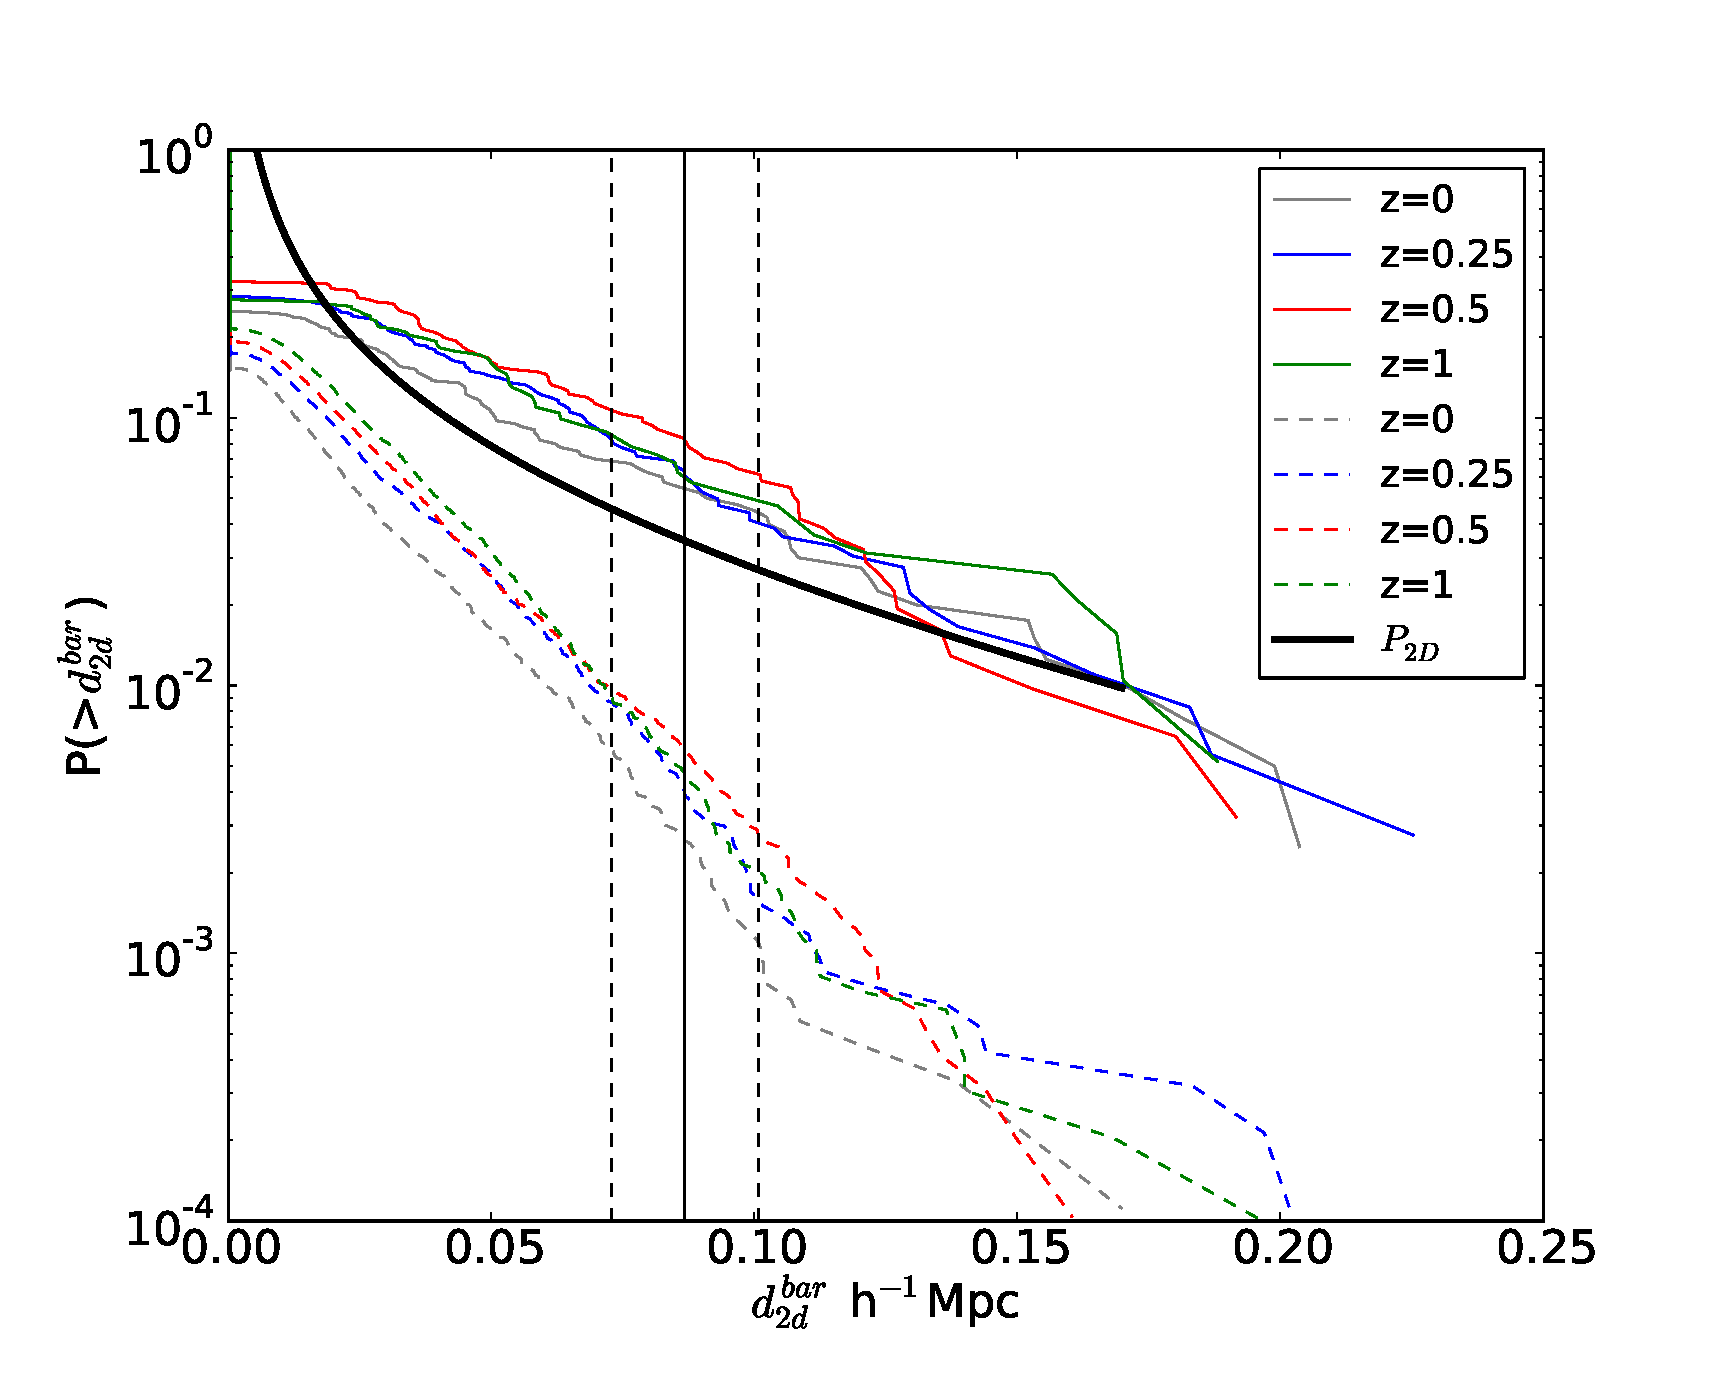
\includegraphics[width=0.5\textwidth]{figure_5.eps}
\end{center}
\caption{Integrated probability distribution for the estimated
  baryonic displacements in the group and cluster samples. Continous (dashed)
  lines correspond to clusters (groups). The continuous black line
  marked as $P_{2D}$ shows the statistics reported by
  \citet{ForeroRomero2010} for a cosmological simulation including DM
  and baryons. The vertical lines correspond to the mean value and
  uncertainty of the displacement measured for \bullg.} 
\label{fig:baryonic_displacements}
\end{figure}


\section{Observational Implications}
\label{sec:observations}


\section{Conclusions}
\label{sec:conclusions}

In this Letter we estimate fraction of galaxy groups and clusters that
can present observational features associated to a bullet-like
event. This is motivated by the recent observational results of
\citep{Gastaldello} where a system (\bullg) on the mass range $1\times
10^{14}$\hMsun and velocity dispersion $650$\kms was reported to
feature a displacement between its baryonic (hot gas) and dark matter
components.  


We estimate the distribution of projected displacements
between the dominant DM clumps in two kinds of systems; groups with
circular velocities $300\kms<V_{\rm c}<700\kms$ and clusters with $V_{\rm
  c}>700$\kms. We report these results at four different redshifts
$z=0.0,0.25,0.5$ and $10$. Our results based on large N-body dark
matter only cosmological simulation with such a resolution that allows
to study the group mass range for the first time in the context of
Bullet-like configurations. 


Our main results is that that a fraction of $50\%$-$60\%$ of the halos
in the group sample present displacement equal or larger than the
observed displacement for \bullg. For halos in the cluster sample this
fraction increases to $80\%$-$85\%$. We also derive an
estimate for the displacement between the DM and the baryonic
component. In the group sample $0.1\%$-$1.0\%$ of the halos show a
displacement equal or larger than  the  measurements of \bullg by
\citep{Gastaldello}. In the cluster sample this fraction rises to
$4\%$-$10\%$. 

We also find distributions for the DM separation and the velocity of
the bullet through its host. If these quantities are normalized by the
virial radius and the circular velocity, respectively, we arrive at
distributions close to universal that are similar for the two halo
samples at all redshifts.

For the case of \bullg the fair comparison is achieved in the cluster
sample, which have statistics dominated by objects of similar mass. In
this case we conclude that the existence of such configuration is
highly probable in $\Lambda$CDM (4$\%$ to $10\%$ abundance). In turn,
for the same separation the fraction for groups is lower (0.1$\%$ to
$1\%$). Taking into account that the difference in spatial abundance between
these two samples is on the order of a factor of $10$, one can
conclude that the absolute number of groups and clusters presenting a DM-baryon
displacement larger or equal to \bullg should be of the same order.

However, an interesting observational possibility opens up with
surveys such as SL2S that can target a large number of groups and
estimate its multi-modal nature from lensing analysis that can be used
as a potential test of $\Lambda$CDM. In this case the absolute number
of groups with a displacement of the same order of \bullg is larger by
a factor of $\sim 8$ than the number of clusters with the same
displacement. 

The CosmoSim database used in this paper is a service by the
Leibniz-Institute for Astrophysics Potsdam (AIP). The  BolshoiP
simulation was performed within the Bolshoi project of the University
of California High-Performance  AstroComputing Center (UC-HIPACC) and
was run at the NASA Ames Research Center. 


\bibliographystyle{apj}
\bibliography{references} 

\end{document}
